\documentclass[11pt]{article}

\usepackage[utf8]{inputenc}  %francais et caractères
\usepackage[T1]{fontenc} 
\usepackage[francais]{babel}

\usepackage{amsmath} %math
\usepackage{amssymb}

\usepackage{version}

\usepackage{graphicx} %images
%\usepackage{caption}
\usepackage{float}
\usepackage{subfig}
%\usepackage{subcaption}
\usepackage{wrapfig} %images dans texte

\usepackage{hyperref} % Hyperlinks

\usepackage[table,xcdraw,dvipsnames]{xcolor} %couleurs
\usepackage{appendix} %annexes
\usepackage{listings} %insertion de lignes de code
\usepackage{physics}
\usepackage{mathtools, stmaryrd}
%\usepackage[framed,numbered,autolinebreaks,useliterate]{mcode}

\usepackage[right=2cm, left=2cm, top=2cm, bottom=2cm, headheight=110pt]{geometry}
\usepackage{lscape}

\usepackage{fancyhdr}
\pagestyle{fancy}
\fancyhf{}
\fancyhead[L]{PR214}
\fancyhead[C]{Rapport Projet Thématique}
\fancyhead[R]{E2}
\cfoot{\thepage}

\usepackage[nottoc]{tocbibind} % Rajoute la bibliographie dans la tdm

%Tables du generateur de tables
\usepackage[normalem]{ulem}
\useunder{\uline}{\ul}{}

\renewcommand\lstlistingname{Code}
\renewcommand{\lstlistlistingname}{Table de Codes}

\lstset{language = C,%
    %basicstyle=\color{red},
    breaklines=true,%{}
    keywordstyle=\color{Orange},
    identifierstyle=\color{Cyan},
    stringstyle=\color{Red},
    commentstyle=\color{Green},
    morekeywords={matlab2tikz},
    morekeywords=[2]{1}, keywordstyle=[2]{\color{black}},
    showstringspaces=false,%without this there will be a symbol in the places where there is a space
    numbers=left,%
    numberstyle={\tiny \color{black}},% size of the numbers
    numbersep=9pt, % this defines how far the numbers are from the text
    emph=[1]{for,end,break},emphstyle=[1]\color{red}, %some words to emphasise
    %emph=[2]{word1,word2}, emphstyle=[2]{style}, 
    backgroundcolor=\color{White},
    basicstyle=\scriptsize\color{black}\ttfamily,
    frame=L,
    captionpos = b,
    %===========================================================
    framesep=3pt,%expand outward.
    framerule=0.4pt,%expand outward.
    xleftmargin=3.4pt,%make the frame fits in the text area. 
    xrightmargin=3.4pt,%make the frame fits in the text area.
    %=========================================================== 
    rulecolor=\color{Red}   
}


\newcommand{\HRule}{\rule{\linewidth}{0.5mm}}

\renewcommand{\arraystretch}{1.5}
\renewcommand{\baselinestretch}{1.5}

\newenvironment{rmq}[1] {\noindent\HRule\par\vspace{5pt}\textbf{\textit{REMARQUE : }}#1}{\\\HRule\par\vspace{5pt}}



\begin{document}

% Page de Garde
\thispagestyle{empty}

\noindent 
DURAND Clovis\hfill{E2} \\ MARINO Xavier\hfill{Mai 2017}
% // et entrer d'autres noms. 



\vspace{1cm}
\begin{center}
\Large{PR 214} % Inserer la matiere concernée
\HRule \\[0.1cm]
{\textsc{\LARGE \textbf{Projet Thématique\\ Conception d'un module en VHDL pour la gestion d'un Pmod OLEDrgb Digilent sur FPGA}}}\\
\HRule\\[01cm]
%\Large{V1.0} % Version of document
\end{center}
\vspace{1cm}

\begin{figure}[htbp]
\begin{center}

\includegraphics[width=10cm]{background.png}
\end{center}
\end{figure}

\vspace{0.5cm}
\begin{center}
\Large{ENSEIRB-MATMECA \\ Bordeaux - Talence}
\end{center}

\vspace{0.5cm}
Encadrant : Yannick Bornat

\newpage
% Tables
\tableofcontents
%\lstlistoflistings
\listoffigures
\newpage 

% Debut doc
\setcounter{section}{-1}

\section{Introduction}

Au cours de ce projet, un objectif clair nous a été fixé : afficher une image sur un écran OLED couleur d'une résolution 96 x 64, connecté sur une carte Nexys4 de Digilent. Cet écran est monté sur un Pmod (extensions de cartes d'interfaces Entrées/Sorties de chez Digilent). Le cœur du projet est de comprendre comment le Pmod communique avec la carte Nexys4 et de lui envoyer les informations nécessaires à son fonctionnement, telle que la séquence de commandes initialisation de l'écran ou les données de l'image que l'on souhaite afficher. \\

\subsection{Segmentation et déroulement du projet}

Le projet a donc été séparé en plusieurs parties. 

D'abord, l'étude du composant et de sa datasheet. En effet, le Pmod de Digilent possède sa propre datasheet, mais sur celui-ci est monté un contrôleur spécifique à l'écran OLED : le SSD1331. Il a donc été nécessaire d’appréhender comment celui-ci fonctionnait. 

Ensuite, nous avons élaboré un programme d'initialisation et d'utilisation de l'écran. Un microprocesseur basique à été implémenté sur FPGA, nous compilions des programmes écrit en langage C, et nous testions le Pmod de cette façon. Ainsi, en se basant sur ce qu'on a appris des datasheet, nous avons mis au point une séquence de commandes pour initialiser l'écran et pour lui envoyer, via la liaison UART de la carte Nexys4 les données bitmap de l'image. Le but de ces programmes est avant tout de comprendre ce qui doit être décrit en VHDL pour le module de gestion de notre écran OLEDrgb, et ils ne constituent pas notre produit fini. 

Enfin, nous avons développé notre module de gestion du Pmod en VHDL. L’environnement de travail choisi est Vivado de Xilinx. En appliquant une ingénierie inverse aux programmes C développés en amont, une architecture précise à été définie, et la conception de tous les blocs composant notre module ont été écrits. \\

En pratique, l'étude de la datasheet à été un travail permanent, et à donc été faite en parallèle au développement de nos programmes C et de nos descriptions VHDL. Les points de fonctionnement de nos composant qui semblent pour certains relativement simples en apparence mais nous ont posé problème tout de même quand nous avancions dans nos études. A chaque problème de la sorte, il a fallu revoir les points concernés de la datasheet à plusieurs reprises. Pour les problèmes plus complexes, comme la gestion de la communication entre la carte et le Pmod, la datasheet à été d'une grande aide. 

\clearpage

\section{Pmod OLEDrgb}

Un Pmod est un périphérique ou extension destinée à être utilisé avec des cartes programmables telles que la Nexys4 de Digilent que nous utilisons dans ce projet. Le Pmod sur lequel notre travail se concentre ici est l'OLEDrgb, un écran OLED (Organic Light-Emitting Diode) \cite{oleddef} d'une résolution de 96 x 64 pixels capable d'afficher 65k couleurs. 

\begin{figure}[H]
\begin{center}
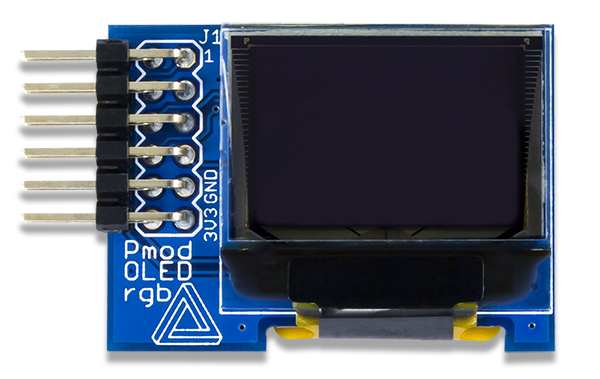
\includegraphics[width = 6cm]{pmodoledrgb-1.png}
\caption{Le Pmod OLEDrgb de Digilent utilisé dans ce projet}
\end{center}
\end{figure}

Pour communiquer avec la carte mère, ce périphérique utilise le protocole SPI (Serial Periphéral Interface Bus). Avec ce protocole, on peut envoyer par paquet les informations et commandes nécessaires au fonctionnement de notre écran OLED. 
Un contrôleur Solomon Systech SSD1331 \cite{ssd1331} est employé pour communiquer entre le Pmod support et le composant de l'écran. Grâce à celui-ci, les commandes envoyées sont exploités et traités. De plus, lorsque que ce contrôleur reçoit des informations, il les stocke dans la RAM de l'écran. Ce contrôleur possède tout un panel de commandes qui permettent d'interagir avec l'écran. (i.e. dessiner un rectangle, un pixel, etc.)\\

Ce Pmod à un connecteur 12 broches qui se branche sur la carte principale :

\begin{figure}[H]
    \begin{center}
        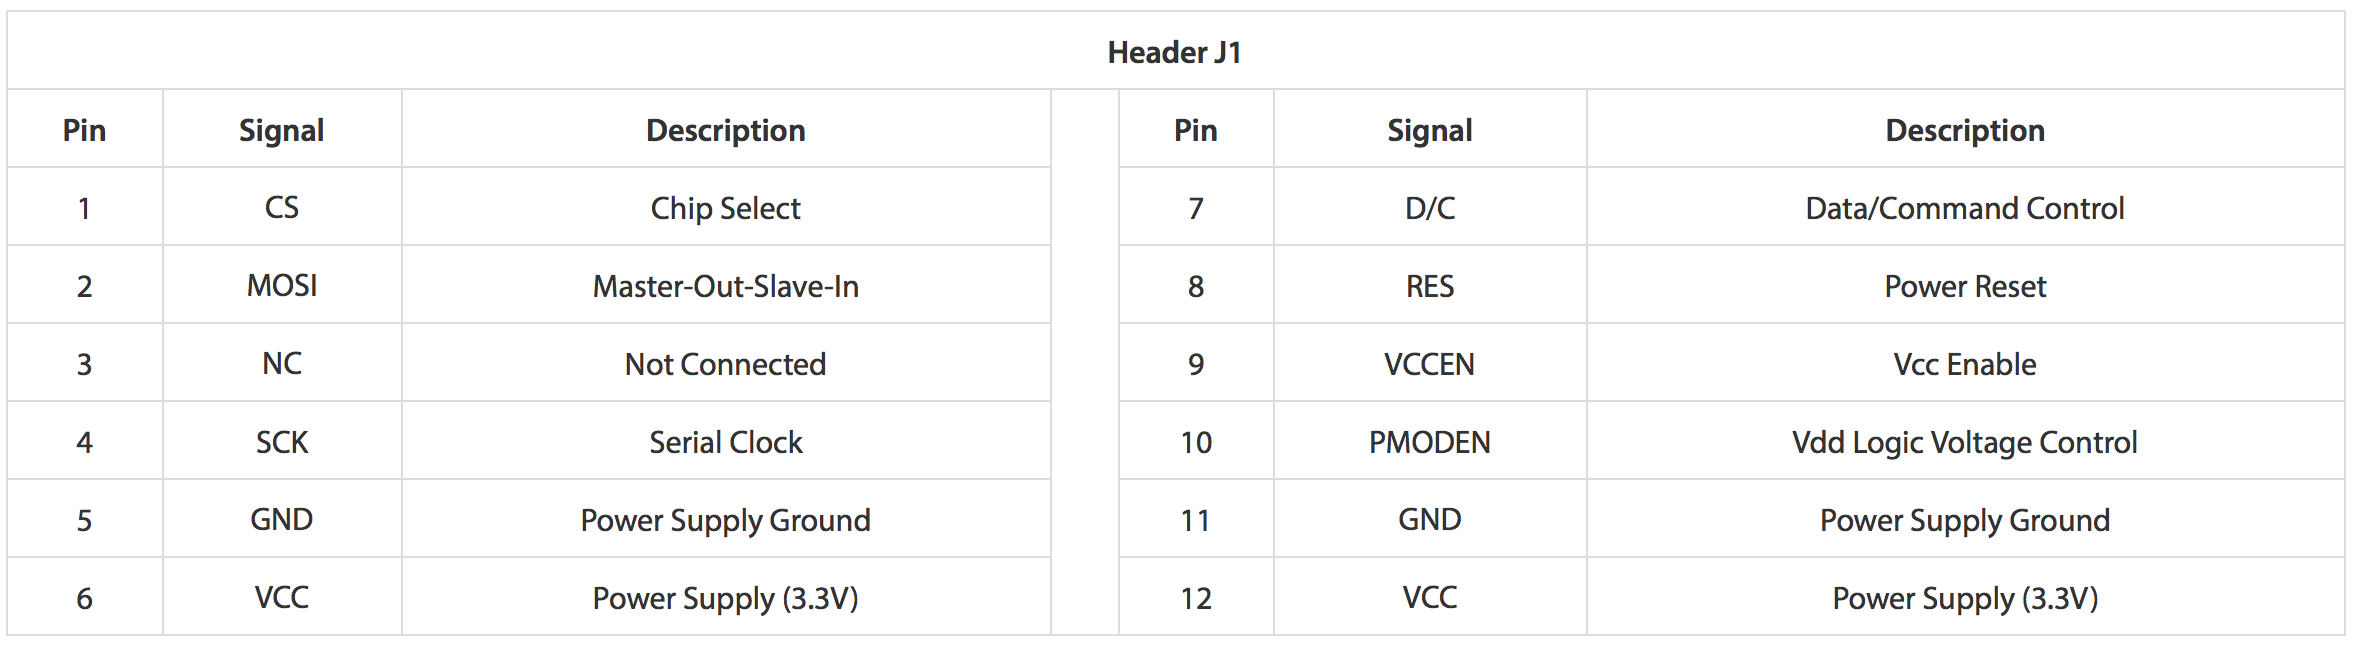
\includegraphics[scale = 0.4, keepaspectratio]{Oled_pin_tab.png}
        \caption{Table de correpsondance des pins du Pmod OLEDrgb \cite{oledrgb}}
    \end{center}
\end{figure}

\begin{comment}
% Generated w/ http://www.tablesgenerator.com/
% Please add the following required packages to your document preamble:
% \usepackage{graphicx}
% \usepackage[table,xcdraw]{xcolor}
% If you use beamer only pass "xcolor=table" option, i.e. \documentclass[xcolor=table]{beamer}
% \usepackage[normalem]{ulem}
% \useunder{\uline}{\ul}{}
\begin{table}[!htbp]
\centering
\resizebox{\textwidth}{!}{%
\begin{tabular}{|c|c|c|c|c|c|c|}
\hline
\multicolumn{7}{|c|}{{\ul \textbf{Header J1}}}                                                                   \\ \hline
Pin & Signal      & Decription             & \cellcolor[HTML]{9B9B9B} & Pin & Signal & Description               \\ \cline{1-3} \cline{5-7} 
1   & CS          & Chip Select            & \cellcolor[HTML]{9B9B9B} & 7   & D/C    & Data/Command Control      \\ \cline{1-3} \cline{5-7} 
2   & MOSI        & Master Out - Slave In  & \cellcolor[HTML]{9B9B9B} & 8   & RES    & Power Reset               \\ \cline{1-3} \cline{5-7} 
3   & \textit{NC} & \textit{Not Connected} & \cellcolor[HTML]{9B9B9B} & 9   & VCCEN  & Vcc Enable                \\ \cline{1-3} \cline{5-7} 
4   & SCK         & Serial Clock           & \cellcolor[HTML]{9B9B9B} & 10  & PMODEN & Vdd Logic Voltage Control \\ \cline{1-3} \cline{5-7} 
5   & GND         & Power Supply Ground    & \cellcolor[HTML]{9B9B9B} & 11  & GND    & Power Supply Ground       \\ \cline{1-3} \cline{5-7} 
6   & VCC         & Power Supply (3.3V)    & \cellcolor[HTML]{9B9B9B} & 12  & VCC    & Power Supply (3.3V)       \\ \hline
\end{tabular}%
}
\caption{My caption}
\label{my-label}
\end{table}
\end{comment}

\clearpage

\section{Fonctionnement du Pmod OLEDrgb}

\subsection{Liaison UART et outils}

Tout d'abord, avant de commencer a envoyer des commandes au contrôleur de l'écran OLED, il faut pouvoir communiquer avec le "processeur" implémenté sur la carte. Une fois cette communication établie, nous pouvons envoyer un programme compilé dans la mémoire du porcesseur, et donc envoyer des commandes à l'écran via l'interface SPI. \\

Ainsi, nous employons la laison UART disponible sur la carte Nexys4 comme bus de communication. Les informations envoyées par cette liaison sont ensuite gérées par le processeur implémenté sur le FPGA. Quand à l'interface côté utilisateur, nous utilisons le logiciel Tera Term (Windows) ou CoolTerm (macOS) pour communiquer avec le port série correspondant à la liason UART établie. \\

Une fois cette communication possible, il s'agit d'écrire un programme en langage C qui permette dans un premier temps de lancer la séquence d'initialisation de l'écran, puis dans un second temps de lui envoyer une image bitmap. 

Pour ce faire, le compilateur xc8 est utilisé. Pour compiler correctement le programme pour notre processeur programmé sur FPGA, nous utilisons les arguments suivants : 
\begin{center}
    \texttt{xc8 --chip=16F636 -m --opt=all -g <NOM SOURCES>}
\end{center}

\begin{rmq}
    Vis à vis du compilateur xc8, le microprocesseur cible est un 16F636. En réalisté, notre cible n'est pas un 16F636, mais un processeur programmé sur FPGA qui ressemble à un processeur 16F636 simplifié. 
\end{rmq}

\subsection{Séquence d'initialisation}

Pour initialiser l'écran correctement, une séquence d'initialisation précise est nécessaire. Pour se renseigner sur la séquence d'initialisation, deux documents sont utiles. 

Le premier est le manuel du Pmod OLEDrgb\cite{oledrgb}. Celui-ci renseigne une séquence d'initialisation type. Cette séquence est la base de notre étude sur l'initialisation. 

Le deuxième est la datasheet du contrôleur SSD1331\cite{ssd1331}. Cette datasheet renseigne tout le jeu de commandes possibles. Ces information sont très utiles car la séquence d'initialisation décrite par Digilent n'est pas complète et des commandes supplémentaires ont du être ajouté à celle-ci. Pour comprendre les commandes dictées par le manuel du Pmod OLEDrgb et pour savoir quelles modifications apporter ou quelles commandes supplémentaires ajouter, le jeu de commandes est essentiel. \\

En C, certaines définitions de constantes et quelques fonctions sont déjà codées dans le but d'envoyer et recevoir des commandes ou des données avec le SPI. Nous nous servirions de ces ressources pour développer notre séquence d'initialisation. 

\begin{enumerate}

    \item La première chose à faire dans la séquence d'initialisation est d'affecter le masque \texttt{OLED\_SPI\_SELECT} au registre \texttt{OLED\_SPI\_STATUS}. Ce masque contient deux informations : La vitesse de l'horloge liée au SPI, puis à l'aide d'un "OU" l'octet \texttt{0x01}. Le bit de poids faible est en réalité lié au "Chip Select" (CS, pin 1, c.f. Figure 2) du Pmod. Si on souhaite communiquer avec le contrôleur via la connectique de la carte Nexys4 et du Pmod, il faut relever le Chip Select. Ainsi, avec cette commande, nous avons défini la valeur de l'horloge du Pmod et la valuer du Chip Select.
    \item Il faut ensuite abaisser le bit de "Data/Commande Control" (DC, pin 7). % Commande ?
    \item On set le bit de "Power Reset" (RES, pin 8). 
    \item On empèche l'alimentation de l'écran - et seulement l'écran - en mettant à $0$ le bit VCCEN ("Vcc Enable", pin 9). 
    \item On met à $1$ le bit PMODEN ("Vdd Logic Voltage Control", pin 10) pour autoriser l'alimentation du Pmod entier. Il faut ensuite faire une temporisation pour attendre que le niveau haut de $3.3\text{V}$ soit bien atteint. La documentation de Digilent conseille 20ms d'attente. Nous avons choisi une temporisation de 100ms. 

    \begin{rmq}
    Dans notre projet, pour cette temporisation ainsi que les suivantes, nous avons souhaité majorer ces valeurs pour s'assurer d'un bon fonctionnement de l'initialisation. Optimiser ces temps est possible, et est une amélioration de ce projet envisageable. 
    \end{rmq}

    \item On clear puis on set le bit RES avec une temporisation de $15 \mu s$ entre les deux actions. Cette opération à pour but de mettre à zéro le contrôleur SSD1331 de l'écran. Ensuite, il faut de nouveau attendre $15 \mu s$ pour attendre que l'opération en question se termine. À partir de ce point, nous pouvons envoyer des commandes au contrôleur via le bus SPI et donc commencer à le configurer. 

    \item Le première commande à envoyer est le déverrouillage de la réception des commandes. On envoi donc 2 octets : \texttt{0xFD} et \texttt{0x12}. Grâce a cette opération, le contrôleur va pouvoir traiter les autres commandes que nous allons lui envoyer. Quand le contrôleur est verrouillé, cette commande est la seule qui peut être interprétée. 

    \item On met l'écran en veille le temps de l'initialisation : \texttt{0xAE}

    \item Ici, on va définir le format de l'image à afficher et des données liées à l'image. La commande varie en fonction de plusieurs paramètres. Il faut d'abord envoyer la commande \texttt{0xA0}. Le second octet règle les paramètres. 

    D'après la datasheet : 
    \begin{itemize}
        \item[-] Les deux bits de poids fort gèrent le format de couleur des données de l'image, c'est-à-dire comment sont codées les couleurs pour un pixel. Nous avons choisi d'utiliser le format de couleur 65k numéro 1. Ces deux bits sont donc égaux à \texttt{0b01}
        \item[-] Le sixième bit permet de "Enable COM Split Odd Even". Il est réglé à 1 conformément aux instructions de Digilent. 
        \item[-] Le cinquième bit permet de régler le ratio de multiplexage de l'écran et comment la RAM est parcourue par le contrôleur pour charger les informations sur l'écran. % XAVIER A L'AIDE
        \item[-] Le quatrième bit permet "d'inverser la gauche et la droite" quand le contrôleur parcours la RAM. Changer ce bit à pour conséquence de donner un effet "miroir" à l'image que l'on souhaite afficher. On le met à 0 pour ne pas avoir cet effet. 
        \item[-] Le troisième bit permet de régler l'ordre des couleurs. Si ce bit est mit à 1, l'ordre est BGR au lieu de RGB. On règle ce bit à 0 pour conserver l'ordre classique RGB. 
        \item[-] Le deuxième bit est celui qui affecte les colonnes 0 à 95 de la RAM aux colonnes 0 à 95 de l'écran. Si ce bit est mis à un, l'affectation est inversée (i.e. 0-95 -> 95-0).
        \item[-] Enfin, le bit de poids faible permet de régler le sens d'incrémentation des adresses : 0 pour une incrémentation horizontale, 1 pour une incrémentation verticale. Nous mettons ce bit à 0. 
    \end{itemize}

    De plus, c'est sur cette commande que l'on règle l'orientation de l'écran. En effet, sur la carte Nexys4, le Pmod OLEDrgb peut être branché à droite ou à gauche. Ce choix est enregistré dans un \texttt{\#define} dans le header \texttt{def.h}. On a donc deux cas : 
    \begin{itemize}
        \item[-] L'écran est branché à droite de la carte. L'orientation est donc "classique", c'est-à-dire que l'orientation est telle que le haut de l'écran correspond avec le haut du Pmod. La commande se résume à l'envoi de deux octets : \texttt{0xA0} et \texttt{0x72} (\texttt{0b01110010}). L'octet de réglage \texttt{0x72} correspond aux réglages explicités bits à bits plus haut. 
        \item[-] L'écran est branché à gauche de la carte. L'orientation est donc dite "inversée", c'est-à-dire que l'orientation est telle que le haut de l'écran correspond avec le bas du Pmod. La commande se résume à l'envoi de deux octets : \texttt{0xA0} et \texttt{Ax60} (\texttt{0b01100000}). Les changements par rapport à l'orientation classique sont d'abord la mise à zéro du bit de réglage du sens de scan des informations pour le remplissage de l'écran, qui se fait dans le sens inverse à présent. Le deuxième changement est la mise à zéro du bit réglant l'affectation des colonnes de la RAM aux colonnes de pixels. Ceux deux changements permettent d'inverser l'orientation de l'écran. Sans l'un de ces changements l'image est déformée car les pixels ne reçoivent pas l'information qui leur est destinée. 
    \end{itemize}

    \item Il s'agit ensuite de définir le pixel de départ de l'écran. La commande \texttt{0xA1, 0x00} permet de définir le pixel en haut à gauche de l'écran (ou en bas à droite si l'orientation est inversée) comme pixel de départ pour l’écriture dans la RAM de l'écran. 

    \item Ensuite l'offset de ligne de l'écran est mis à zéro par la commande \texttt{0xA2, 0x00}. 

    \item Le ratio de multiplexage est réglé à 64, conformément aux instruction de Digilent, avec les commandes \texttt{0xA8, 0x3F}. De cette façon, toutes les broches de multiplexage sont activées. 

    \item On choisit ensuite d'alimenter le contrôleur et l'écran via une source d'énergie externe. Autrement dit, on choisit un $V_{CC}$ externe. Le $V_{CC}$ en question est celui de la carte Nexys4 dans notre cas. LA commande correspondante est \texttt{0xAD, 0x8E}. 

    \item Conformément aux instructions de Digilent, on règle la période de l'horloge de l'affichage avec la commande \texttt{0xB1, 0x31}. 

    \item Le ratio de division de l'horloge de l'affichage et la fréquence de l'oscillateur interne sont réglés à leur valeur maximale avec la commande \texttt{0xB3, 0xF0}

    \item Le contraste est réglé par 3 suites de commandes concernant les trois couleurs : rouge (\texttt{0x8A, 0x64}), vert (\texttt{0x8B, 0x78}), bleu (\texttt{0x8C, 0x64}). 

    \item Le niveau de précharge des broches de l'écran est mis à 45\% du niveau de $V_{CC}$ comme indiqué par le manuel de Digilent. 

    \item 


\end{enumerate}


\subsection{Envoi de données}

Après nous êtres familiarisé avec certaines commandes du microcontrôleur, s'est posé à nous la problématique d'envoi de donnée à l'écran OLEDrgb. Tout comme les commandes, les données sont envoyées en SPI sous la forme d'octet. Une fois les commandes de début et de fin d'écriture dans la RAM du Pmod, envoyées, nous avons pu directement écrire dans cette RAM et ainsi afficher les couleurs voulues sur l'écran, en passant le signal \texttt{DC} au niveau haut. Le microcontrôleur fonctionne avec un système de codage RGB de 16 bits, soit 5 bits pour le rouge puis 6 bits pour le vert et enfin 5 bits pour le bleu, du bit de poids fort au bit de poids faible. Ainsi il nous faut envoyer deux octets en SPI afin d'allumer un pixel à la couleur voulu. 

Afin d'afficher une image complète sur l'écran, il nous faut convertir une fichier image source, \texttt{.bmp}, en un fichier texte compréhensible par le pic implémenté sur la carte NEXYS4. Pour ce faire nous avons utilisé le langage Pyhton. Le programme de conversion, \texttt{bmp\_to\_hex.py}, fonctionne comme suit : 
\begin{itemize}
\item[\textbullet]
Tout d'abord, on crée un fichier texte qui sera notre sortie.
\item[\textbullet]
Dans un second temps on vient charger l'image à convertir, celle-ci est désormais stockée dans une matrice à trois dimension. Elle possède 96x64x3 éléments, un code RGB pour chaque pixel. À noter que le fichier \texttt{.bmp} initial est déjà de la taille 96x64.
\item[\textbullet]
Puis on vient ramener le code RGB contenu dans matrice au format voulu. En effet, chaque composante possèdent intialement 256 états différents, il nous faut ramener le bleu et le rouge à 32 et le vert à 64.
\item[\textbullet]
On parcours ensuite la matrice en inscrivant dans le fichier texte les différents octets rencontrés. Puisqu'il nous faut concatener 5 bits et 3 bits provenant respectivement des codes R et G d'un pixel, puis 3 bits et 5 bits provenant des codes G et B, afin de synthétoser nos octets, le code est à peu délicat, nous ne rentrerons pas plus dans les détails.
\end{itemize}
Puisque le convertisseur ainsi programmé fonctionne en inscrivant des charactères dans un fichier texte, nous avons pu le configurer en fonction de nos besoins et de nos éssais. À terme il nous également permis de générer les données en hexadécimal à stocker dans nos sources VHDL.

Ainsi en envoyant le fichier texte via la liaison UART du microprocesseur, nous avons pu récupérer chacune des données inscrites afin de les envoyer vers le Pmod OLEDrgb.

\newpage

\section{Module de gestion du Pmod OLEDrgb}

Une fois les différentes séquences de commandes mises en place, nous sommes passé à la description en langage VHDL du module de gestion de l'écran OLED. Ce développement s'est scindé en la description de quatre modules :

\begin{itemize}

\item[\textbullet] \texttt{SPI\_controller} : Ce module générè l'ensemble des signaux nécessaires à la transmission d'informations par le biais du protocole SPI.

\item[\textbullet] \texttt{MEM\_init} : Cette source est une ROM contenant les commandes d'initialisations du microcontrôleur.

\item[\textbullet] \texttt{RAM} : Cette RAM contient les données de l'image à afficher sur l'écran, elle est à l'image de la RAM présente dans le microcontrôleur. Cependant elle a été décrite avec deux accès pour permettre son utilisation par un utilisateur extérieur.

\item[\textbullet] \texttt{FSM} : Cette machine d'état conditionne l'envoi des données d'initialisation stockées dans la ROM vers le module SPI, puis celui de l'image stockée dans la RAM.

\end{itemize}

Les deux mémoires présentées plus haut sont toutes deux composées de données sur 16 bits. Ce format a été choisi car il correspond, pour la RAM, au format de données pour un pixel de l'écran. La RAM est combinatoire en lecture et séquentielle pour l'écriture. L'implémentation de deux horloges distinctes, même si  elles sont toutes deux reliées à la même horloge de fonctionnement de la carte, a été nécessaire à la synthèse d'une RAM à double entrée. La ROM quant à elle est purement combinatoire.

\subsection{Module de transmission de données destinées à un protocole d'envoi SPI}

\subsubsection{Principe de fonctionnement du module}

Le protocole de communication SPI permet la transmission de bus de données de 8 bits par le signal \texttt{MOSI} (Master Out Slave In), c'est le signal d'horloge \texttt{sclk} qui permet la lecture des différentes bits du \texttt{MOSI}. En effet, c'est le déclenchement de huit périodes d'horloge qui permet au contrôleur de détecter l'envoi de données. Le protocole SPI possède également une entrée de contrôle \texttt{CS} (Chip Select) et un signal de retour \texttt{MISO} (Master In Slave Out). L'ensemble des signaux sont représentés dans la figure suivante, représentant la caractéristique simplifiée d'un envoi de données par SPI.

\begin{figure}[H]
\begin{center}
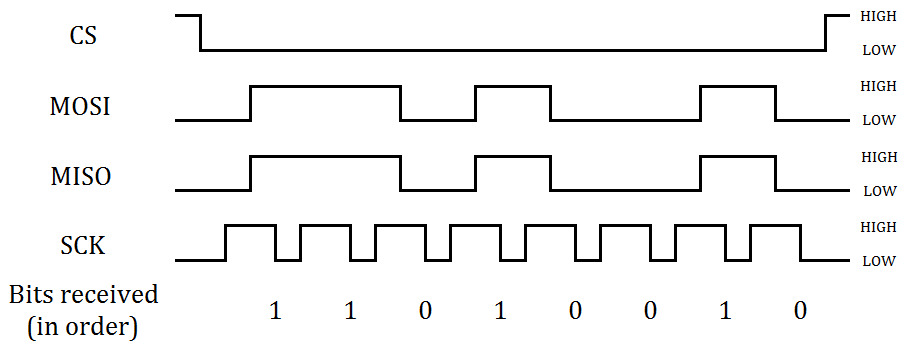
\includegraphics[scale = 0.32, keepaspectratio]{spi_signals.png}
\caption{Chronogramme simplifié du fonctionnement du protocole SPI \cite{spiimg}}
\end{center}
\end{figure}

Dans le cas du microcontrôleur SSD1331, la lecture des bits de données est faite sur front montant de \texttt{sclk}. Nous avons pu également tester, lors de notre phase de recherche, qu'aucun passage à l'état logique haut n'était nécessaire pour l'entrée \texttt{CS} entre deux envois de données. Enfin, c'est le bit de poids fort qui est envoyé en premier au contrôleur lors de la transmission d'un octet. À l'aide de l'ensemble des ces informations nous avons pu décrire le module explicité plus haut.

La source prend en entrée les signaux \texttt{clk} et \texttt{reset} communs à tous bloc séquentiels, la donnée d'entrée sur 8 bits, ainsi qu'un signal logique d'activation qui dure une période d'horloge. En sortie, sont générés les signaux nécessaires à la communication en SPI, ainsi qu'un signal logique $busy$ qui permettra par la suite de temporiser l'envoi de données.

D'après la datasheet du microcontrôleur, la fréquence de fonctionnement du module SPI ne doit pas dépasser les 6 MHz.

\begin{eqnarray*}
&&f_{max} = 6\text{ Mhz}\\
&\Rightarrow&T_{min} = \frac{1}{6}\text{ }\mu\text{s}\\
&\Rightarrow&T_{haut_{min}} = \frac{1}{12}\text{ }\mu\text{s} \sim 83.33\text{ ns}
\end{eqnarray*}

Nous avons donc choisi, le premier entier paire, afin d'avoir un signal \texttt{sclk} de rapport cyclique 0.5, satisfaisant la condition précédente, comme facteur de division de la fréquence de fonctionnement principale. La fréquence de fonctionnement de la carte NEXYS4 étant 100 Mhz, l'entier choisit est donc 18.


\subsubsection{Description et fonctionnement technique}

La description se subdivise en plusieurs processus séquentiels qui génèrent chacun une sortie du module en fonction des entrées. 

\begin{itemize} 

\item[\textbullet] \texttt{sclk} : À chaque détection d'un signal d'$enable$, huit périodes d'horloge, d'une fréquence de 100/18 Mhz, sont générés par le biais de deux compteurs. Le premier, \texttt{cpt\_sclk}, est majoré par la constante définie plus haut et impose la fréquence de \texttt{sclk}. Le second, \texttt{cpt\_octet}, dénombre le nombre de coup d'horloge déjà générés, il est donc majoré par 8. Cette horloge permettra de séquencer l'envoi successif des 8 bits de données. Le niveau de repos de l'horloge devant être reçu par le microcontrôleur étant le niveau haut et la lecture du bit de donné étant effectuée sur front montant de l'horloge, il nous faut envoyer, en sortie du module, l'inverse du signal ainsi généré.

\item[\textbullet] \texttt{SPI\_busy} : Le signal d'occupation reste au niveau haut durant les huit périodes "actives" de \texttt{sclk}, le reste du temps il est maintenu à 0.

\newpage

\item[\textbullet] \texttt{MOSI} : À chaque détection d'un signal d'$enable$, la donnée d'entrée est sauvegardée dans une registre à décalage. Ce registre à décalage est incrémenté à chaque front montant de \texttt{sclk} et c'est sa valeur qui est lue afin de mettre à jour le signal de sortie. Dans la source \texttt{SPI\_controller.vhd}, le dernier processus, qui permet l'actualisation du signal \texttt{MOSI}, a été décrit de façon séquentielle. Le signal \texttt{sdata\_in} étant déjà séquentiel et le signal de sortie seulement lu lors de l'activation de \texttt{sclk}, le processus aurait pu être décrit de manière combinatoire. Cependant, la fréquence de fonctionnement du SPI étant très faible devant celle de la carte, ce choix n'a très peu d'impact sur l'optimisation du temps de transmission et aucun sur le bon fonctionnement du module.

\end{itemize}

Une fois la description terminée, nous avons pu déboguer le code à l'aide de l'outil de simulation de Vivado, duquel est tiré le chronogramme présent en figure X, représentant le fonctionnement du module.

\begin{figure}[H]
\begin{center}
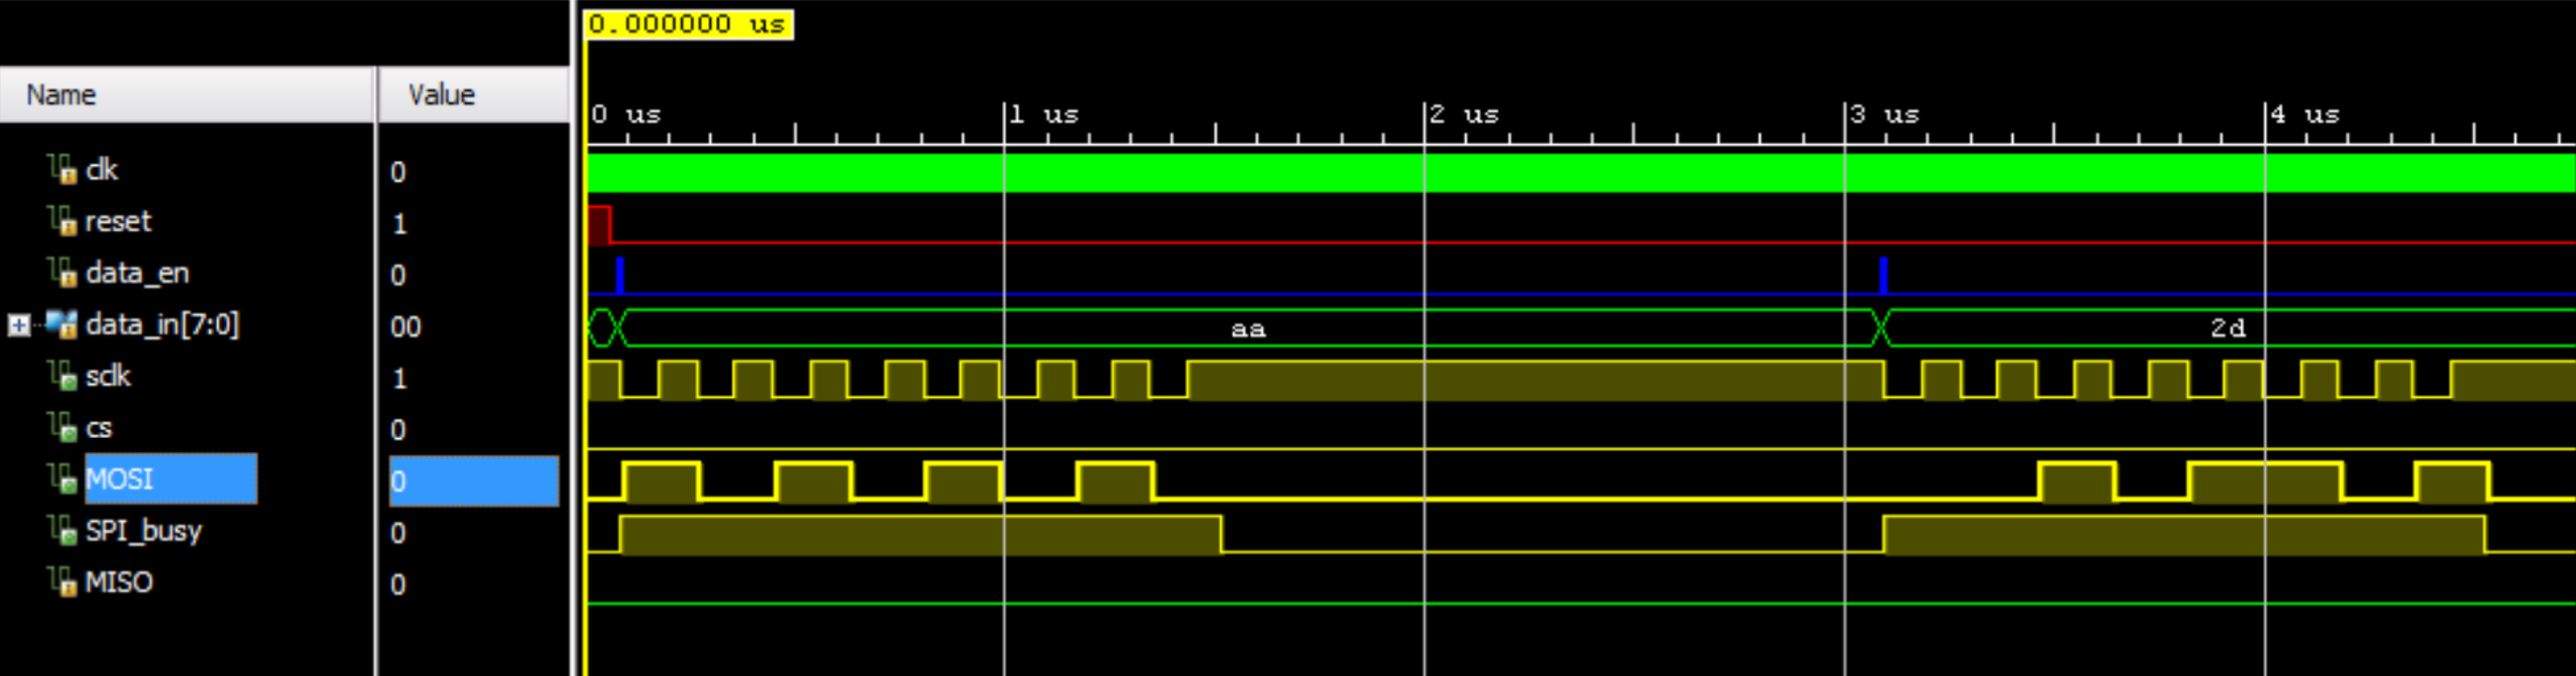
\includegraphics[scale = 0.3, keepaspectratio]{chrono_SPI_controller.png}
\caption{Chronogramme du module \texttt{SPI\_controller}}
\end{center}
\end{figure}

\subsection{Contrôle d'envoi de commandes et de données}

\subsubsection{Principe de fonctionnement de la machine d'état}

Une fois le module de communication SPI terminé, nous nous sommes penché sur la machine d'état qui aura pour rôle d'ordonnancer les différentes étapes du processus d'initialisation, puis l'envoi des données de l'image. En effet, la séquence d'initialisation déterminée plus tôt peut être subdivisée en plusieurs étapes successives :

\begin{itemize}

\item[\textbullet] Le changement d'état des différentes pins de contrôles du Pmod (\texttt{DC}, \texttt{RES}, \texttt{VCCEN} et \texttt{PMODEN}), séparé ou non par des temporisations. Ces étapes occuperons les états 1 à 6, puis 10 de la machine d'état.

\item[\textbullet] Une séquence d'envoi de commandes par le biais du protocole SPI. Ces commandes, au nombre de quarante-quatre, sont stockés dans la mémoire évoquée plus haut.

\item[\textbullet] Et enfin la commande d'allumage de l'écran qui est la dernière étape de l'initialisation.

\end{itemize}

Nous avons ensuite fait le choix de faire suivre l'initialisation par un tracé de rectangle en utilisant les différentes commandes du microcontrôleur, afin de vérifier le bon focntionnment de la séquence précédente. En effet, la RAM du Pmod étant nettoyée par nos précédentes utilisation, nous n'avions aucun retour visuel de l'allumage de l'écran.

Enfin, la dernière étape consiste à venir chercher les données de l'image de la RAM de notre module vers celle du contrôleur.La figure X illustre la machine d'état ainsi mise en place, dans un schéma simplifié, sans les différentes conditions de changement d'état.

\begin{figure}[H]
\begin{center}
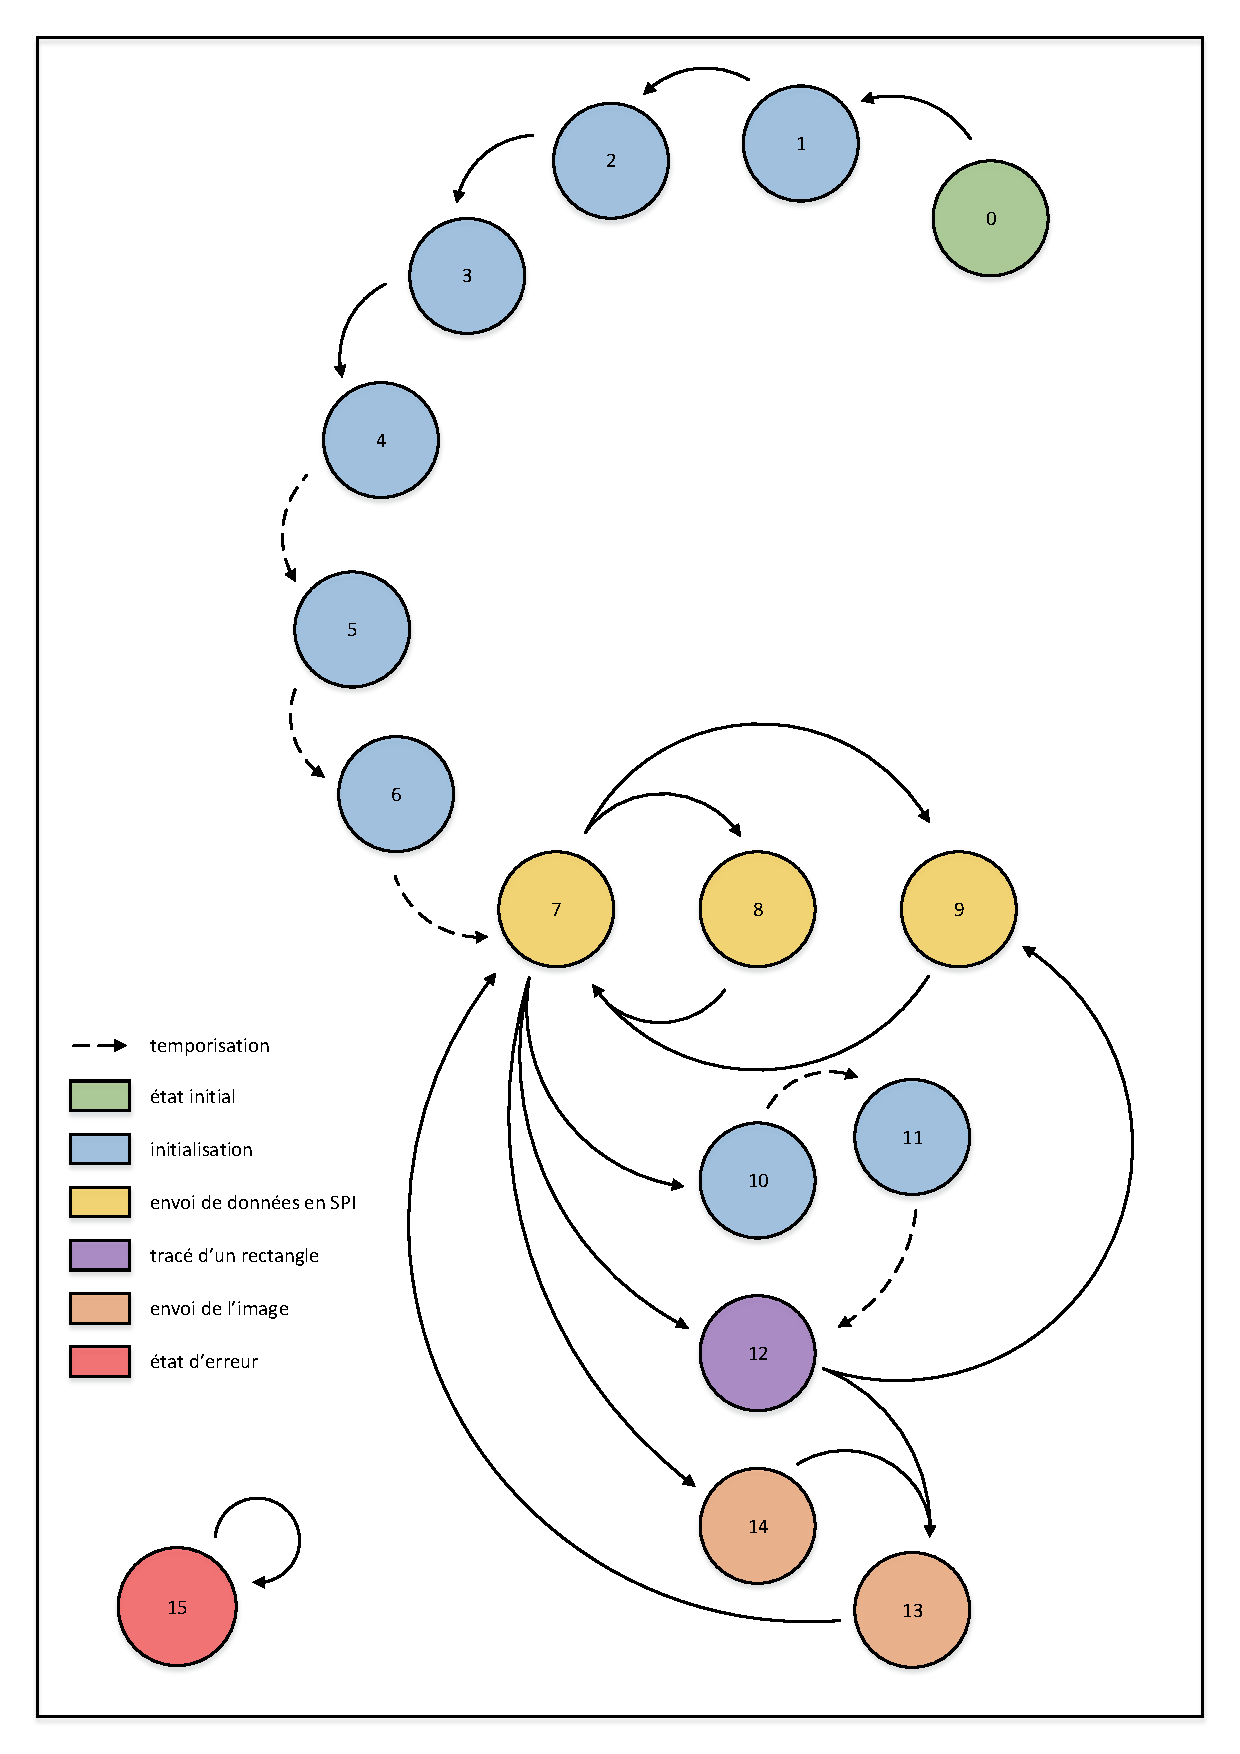
\includegraphics[scale = 0.67, keepaspectratio]{fsm_visio.pdf}
\caption{FSM du module de contrôle du Pmod OLEDrgb}
\end{center}
\end{figure}

\subsubsection{Description de la machine d'état}

La machine d'état est composée d'un processus séquentiel qui détermine l'état présent et d'un processus combinatoire qui détermine l'état futur en fonction de l'état présent, des entrées du module et d'un ensemble de signaux internes à la source. L'ensemble des processus qui suivent les deux premiers, sont destinés à générer l'ensemble des signaux de sorties et internes de la FSM, c'est sur ces derniers que nous allons nous pencher.

\begin{itemize}

\item[$\rightarrow$] \textbf{Les compteurs}

\begin{itemize}

\item[\textbullet] \textbf{Les temporisations} : Afin de satisfaire les différentes temporisations nécessaires à la séquence d'initialisation, nous avons synthétisé trois compteurs permettant la modélisation de trois temporisations d'une durée de 500 ms, 150 ms et 15 $\mu$s. Trois processus permettent donc d'incrémenter les différents compteurs dans les états correspondants. Ces derniers ne peuvent être quittés seulement lorsque le compteur atteind sa valeur maximale. Tout come pour la synthèse de \texttt{sclk}, la valeur maximale des compteurs est déterminée grâce à la fréquence de fonctionnment de la carte NEXYS 4.

\item[\textbullet] \textbf{Les indices de lecture} : L'état numéro 7 de la machine d'état correspond au temps d'occupation du module lors de l'envoi d'un octet en SPI. Entre deux envois de données et donc deux passages à l'état 7, on vient incrémenter l'indice de lecture de la mémoire en cours de lecture, c'est l'état 9 qui se charge de cela. L'état 8 quant à lui, permet l'incrémentation d'un compteur modulo 2 qui désigne successivement les deux octets compris dans une case mémoire. Ainsi, trois processus incrémentent respectivement les compteurs \texttt{read\_idx\_mem}, \texttt{read\_idx\_ram} et \texttt{cpt\_read}. À noter que le compteur \texttt{read\_idx\_mem} possède deux valeurs d'arrêt, puisqu'une partie la mémoire est utilisée pour stocker les commandes d'initialisation et une autre pour les commandes de tracé de rectangle. Ces commandes peuvent d'ailleurs être inhibées dans le code vhdl car inutiles à l'initialisation.

\end{itemize}

\item[$\rightarrow$] \textbf{Les signaux de sortie}

\begin{itemize}

\item[\textbullet] \textbf{Vers le Pmod} : Les processus qui suivent ont pour rôle de $set$ ou $reset$ les signaux de contrôle du Pmod \texttt{DC}, \texttt{RES}, \texttt{VCCEN} et \texttt{PMODEN}, en fonction de l'état présent.

\item[\textbullet] \textbf{Vers le module SPI} : Enfin, les trois derniers processus permettent la bon focntionnement du module SPI. En effet l'un d'eux génère le signal \texttt{data\_en} nécessaire à la tranmission de donnée par le module SPI, ce signal est condionné selon un signal \texttt{flag\_en} synthétisé juste avant. Ce dernier est presque à l'image du signal \texttt{SPI\_busy}, cependant il passe au niveau haut un coup d'horloge avant \texttt{SPI\_busy}, ce qui permet à \texttt{data\_en} d'être au niveau haut seulement pendant une période d'horloge. Comme l'illustre la figure X.

\begin{figure}[H]
\begin{center}
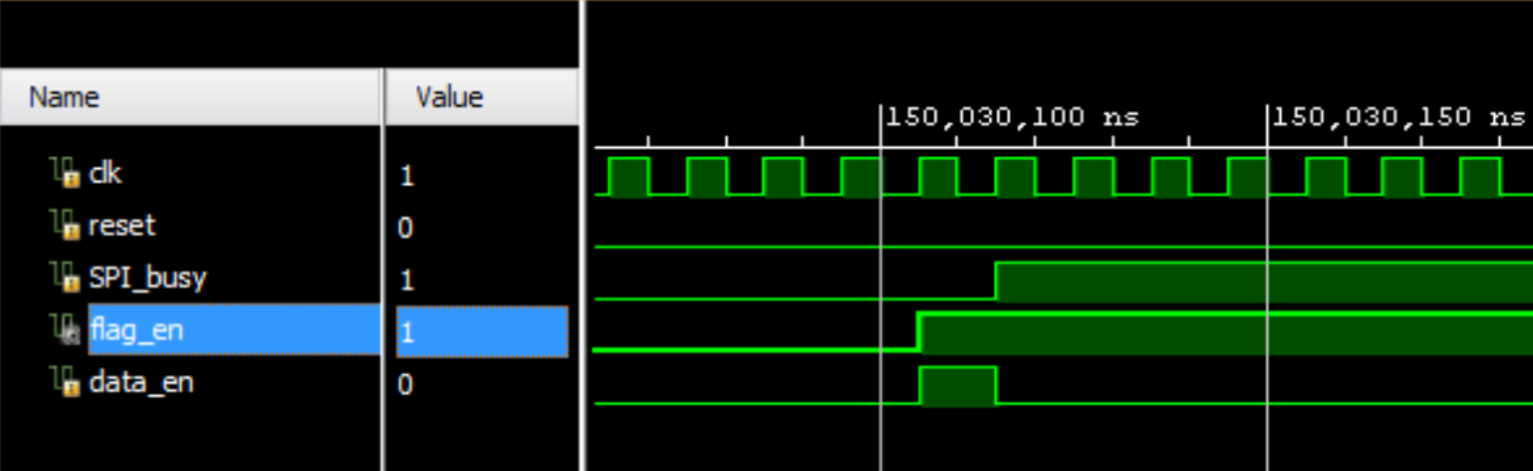
\includegraphics[scale = 0.4, keepaspectratio]{chrono_flag_en}
\caption{Chronogramme représentant le rôle de \texttt{flag\_en}}
\end{center}
\end{figure}

Le dernier processus est un processus combinatoire, qui, en fonction de \texttt{DC} et \texttt{cpt\_read}, vient relier la sortie de la FSM et donc l'entrée du module SPI, au bon octet de la ROM ou de la RAM. Ce fonctionnnment est illustré dans la figure qui suit.

\begin{figure}[H]
\begin{center}
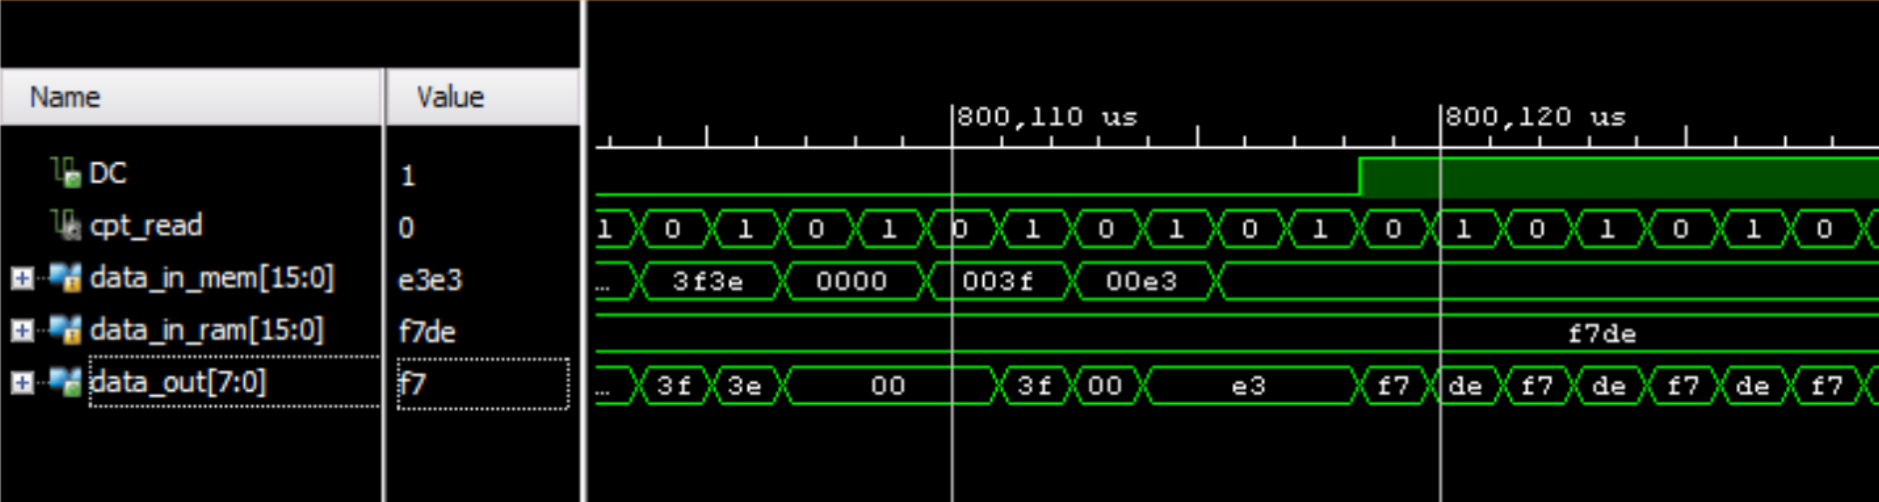
\includegraphics[scale = 0.4, keepaspectratio]{chrono_out}
\caption{Évolution de \texttt{data\_out} en dfonction des différents paramètres}
\end{center}
\end{figure}

On peut voir que, dès que l'envoi de commandes passe en envoi de données, la sortie est reliée à la RAM et non plus à la ROM. Les deux octets de chaque case mémoire sont bien lus grâce au changement d'état de \texttt{cpt\_read}.

\end{itemize}

\end{itemize}

Une fois l'ensemble des composants décrits, nous avons pu les instancier et ainsi simuler le fonctionnement globale du module de gestion de l'écran.

\begin{figure}[H]
\begin{center}
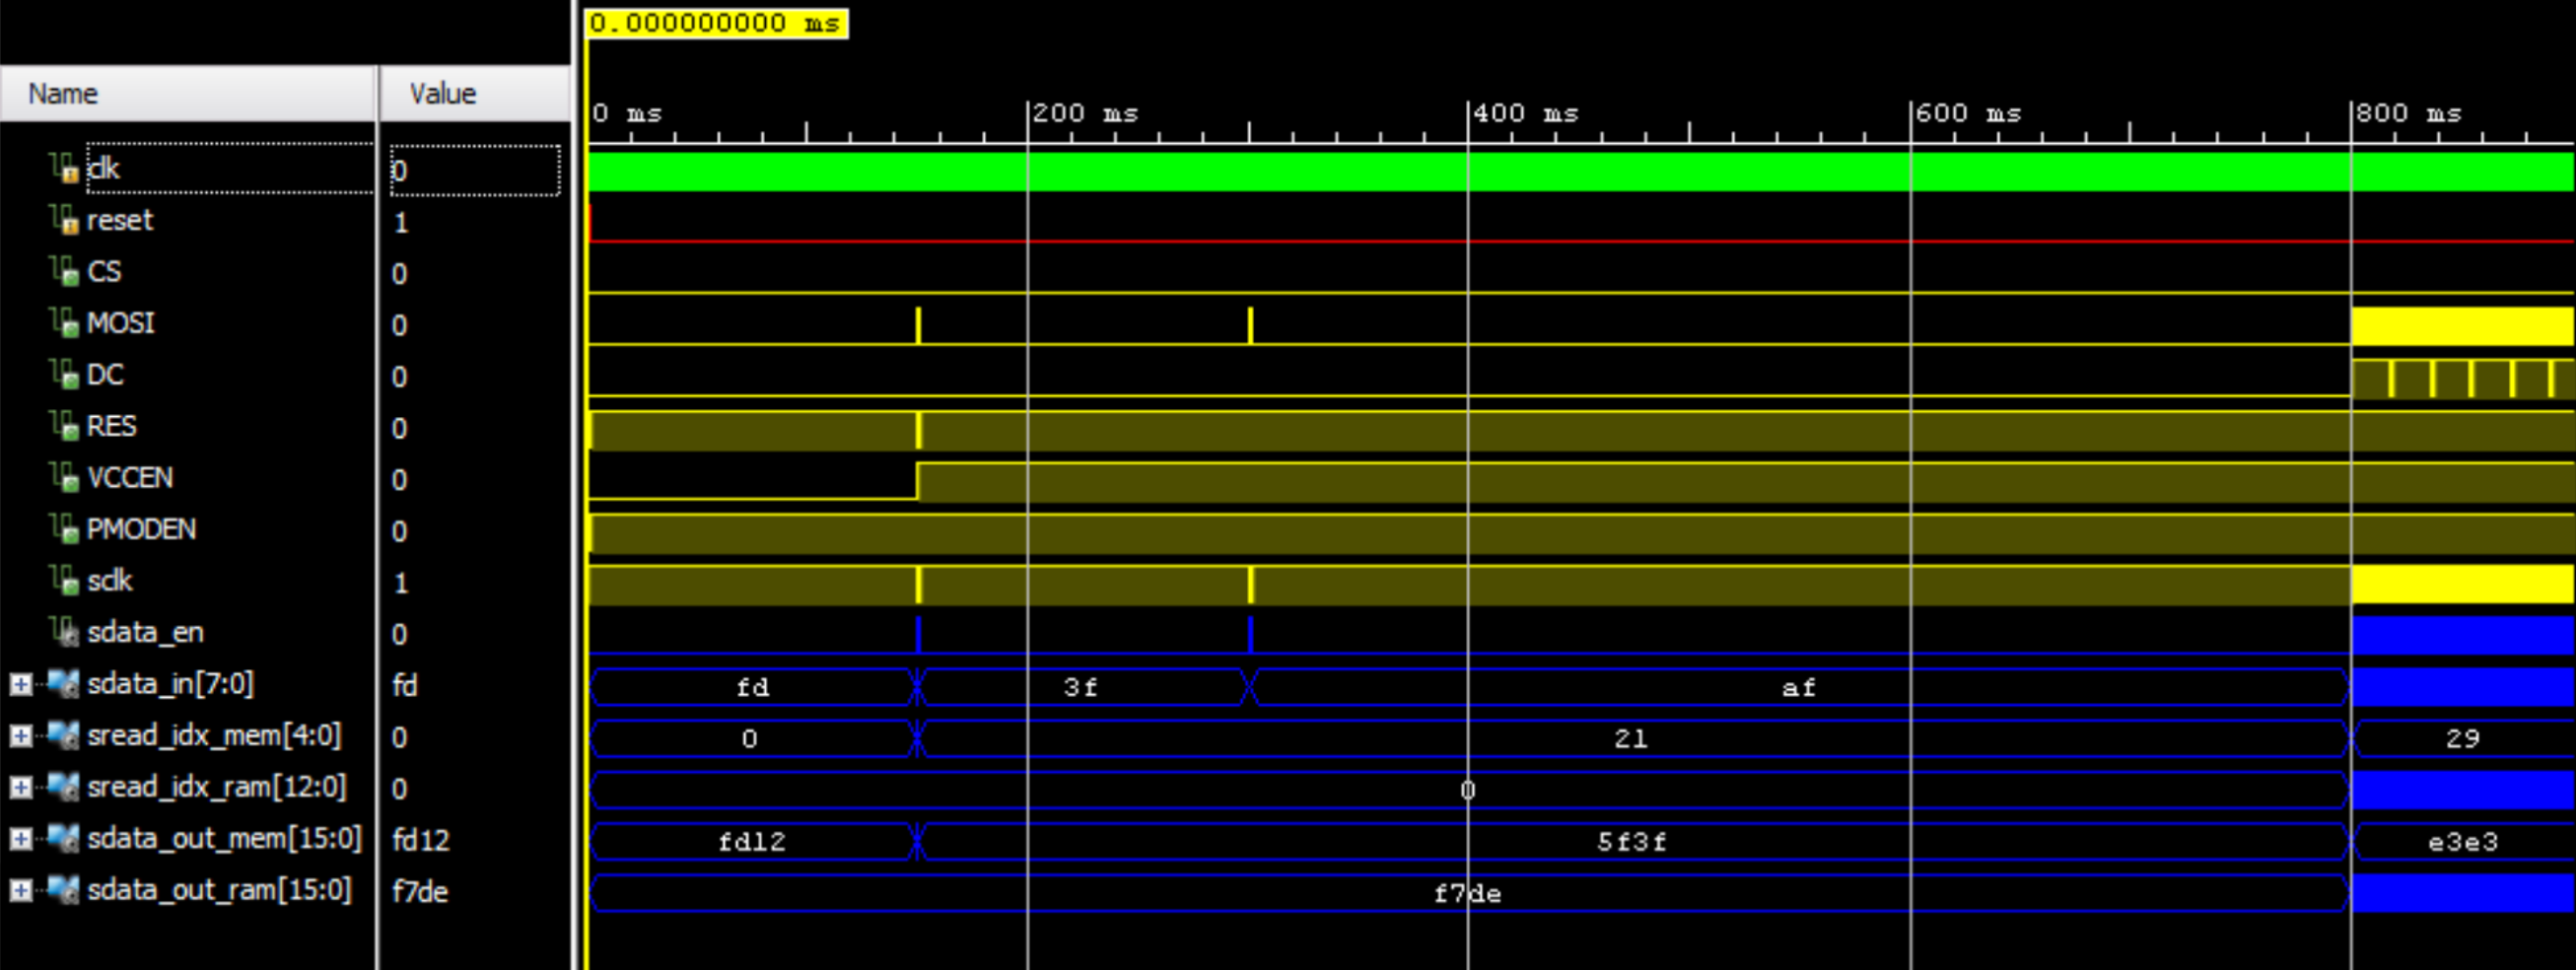
\includegraphics[scale = 0.3, keepaspectratio]{chrono_1}
\caption{Chronogramme représentant l'ensemble de la séquence synthétisée}
\end{center}
\end{figure}

Sur la figure précente on peut voir au niveau du signal \texttt{MOSI} les différentes étapes d'initialisation. Après environ 150 ms nécessaire à la prise en compte des commutations des signaux de commmandes, au premier pic se trouve l'envoi des commandes d'initialiation via le protocole SPI. Ensuite, après de nouveau environ 150 ms, se trouve le second pic qui correspond à la commandes d'allumage. Enfin, après un temps d'attente de 500 ms, on peut relever un travail continu au niveau du signal \texttt{MOSI}, il s'agit de l'envoi des commandes de tracé du rectangle, puis le rafraichissement continu de l'écran.

Dans les deux figures qui suivent, qui sont un zoom de la précédente, on peut mieux se rendre compte du protocole d'envoi des commandes durant l'initialisation et ainsi vérifier son fonctionnnement.

\begin{figure}[H]
\begin{center}
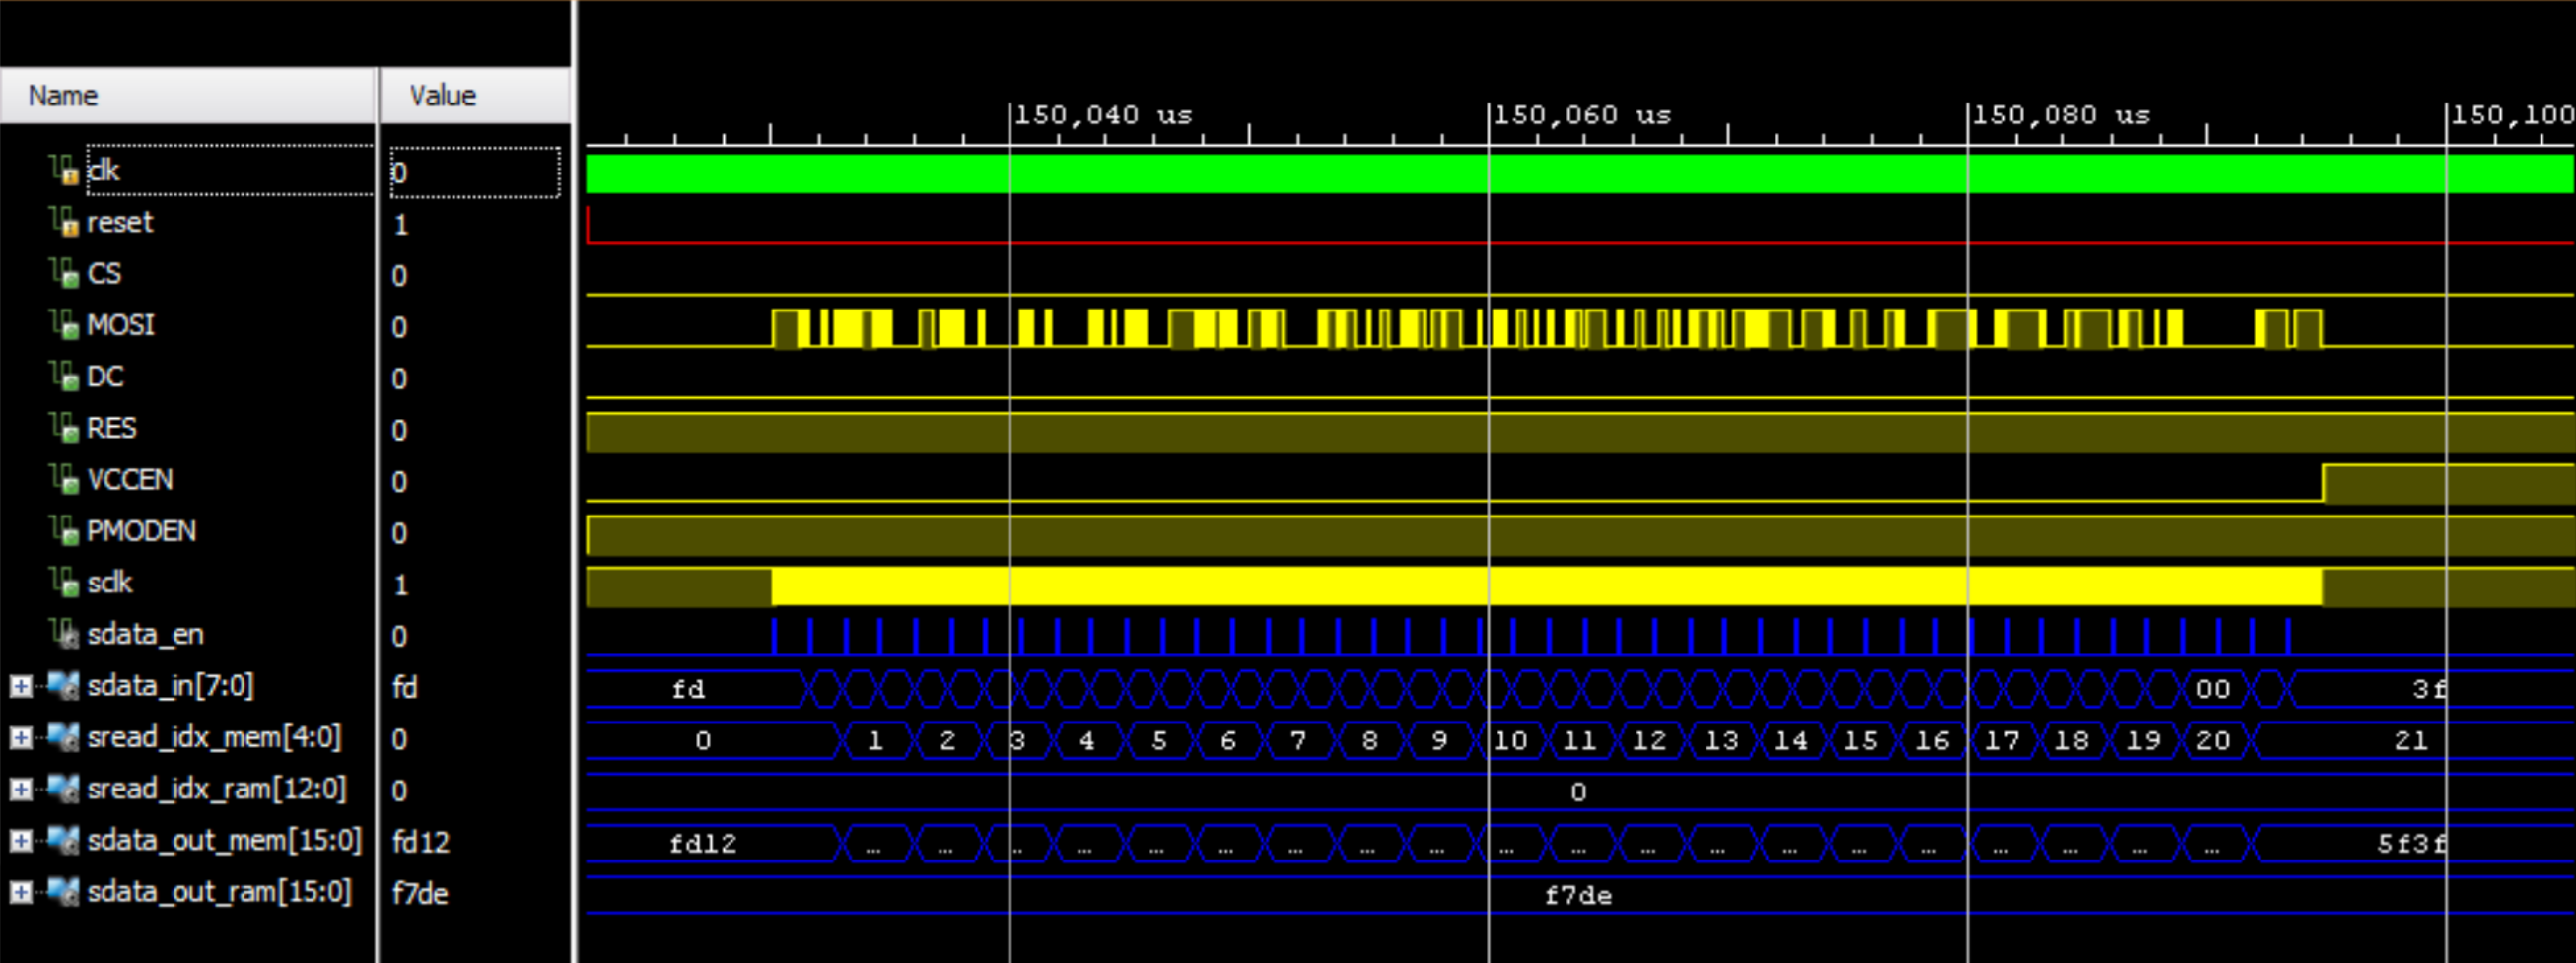
\includegraphics[scale = 0.3, keepaspectratio]{chrono_2}
\caption{Zoom sur l'envoi des commandes d'initialisation}
\end{center}
\end{figure}

\begin{figure}[H]
\begin{center}
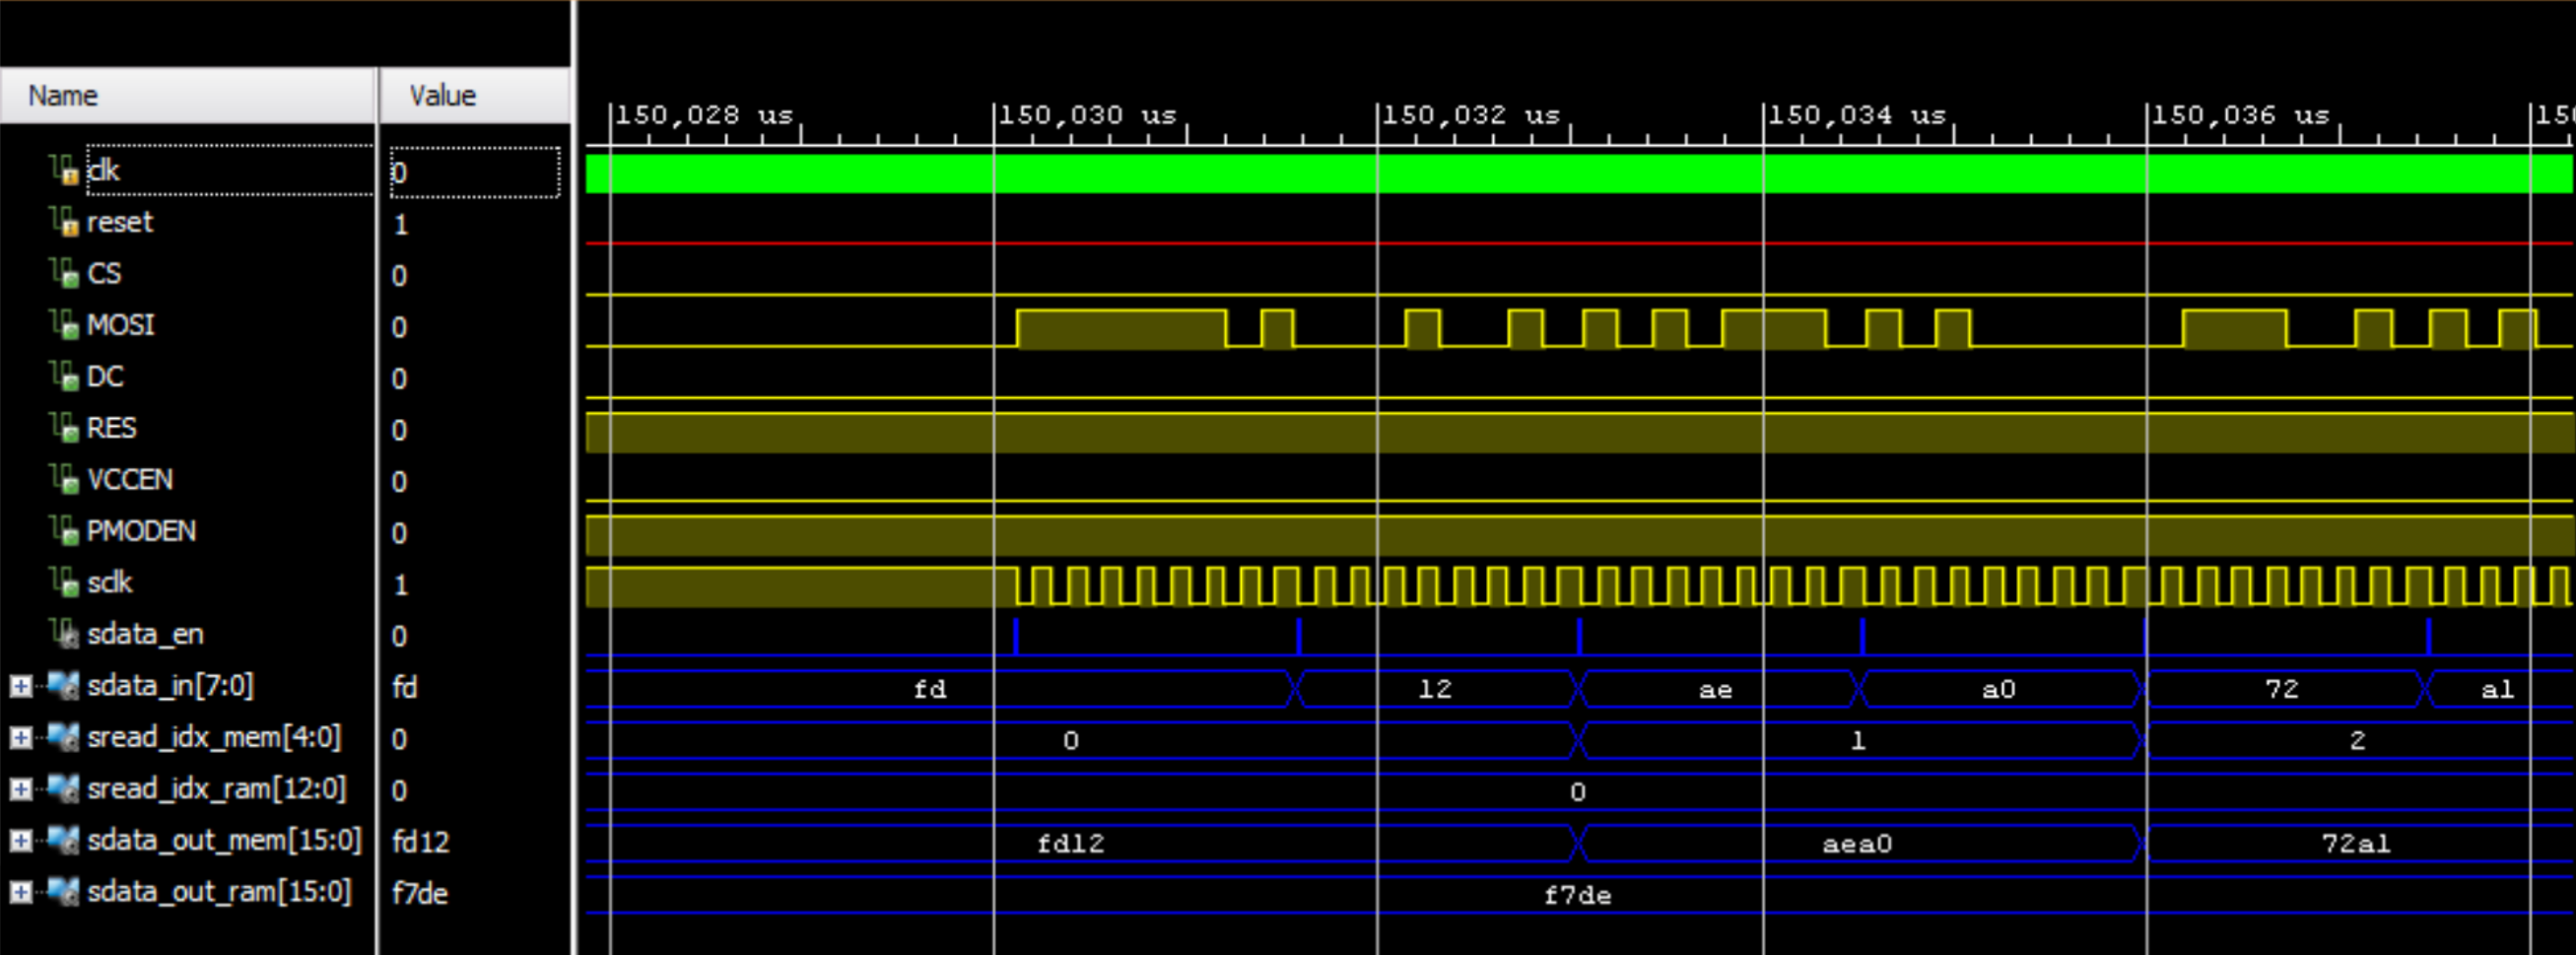
\includegraphics[scale = 0.3, keepaspectratio]{chrono_3}
\caption{Zoom sur la première commande d'initialisation}
\end{center}
\end{figure}

\begin{figure}[H]
\begin{center}
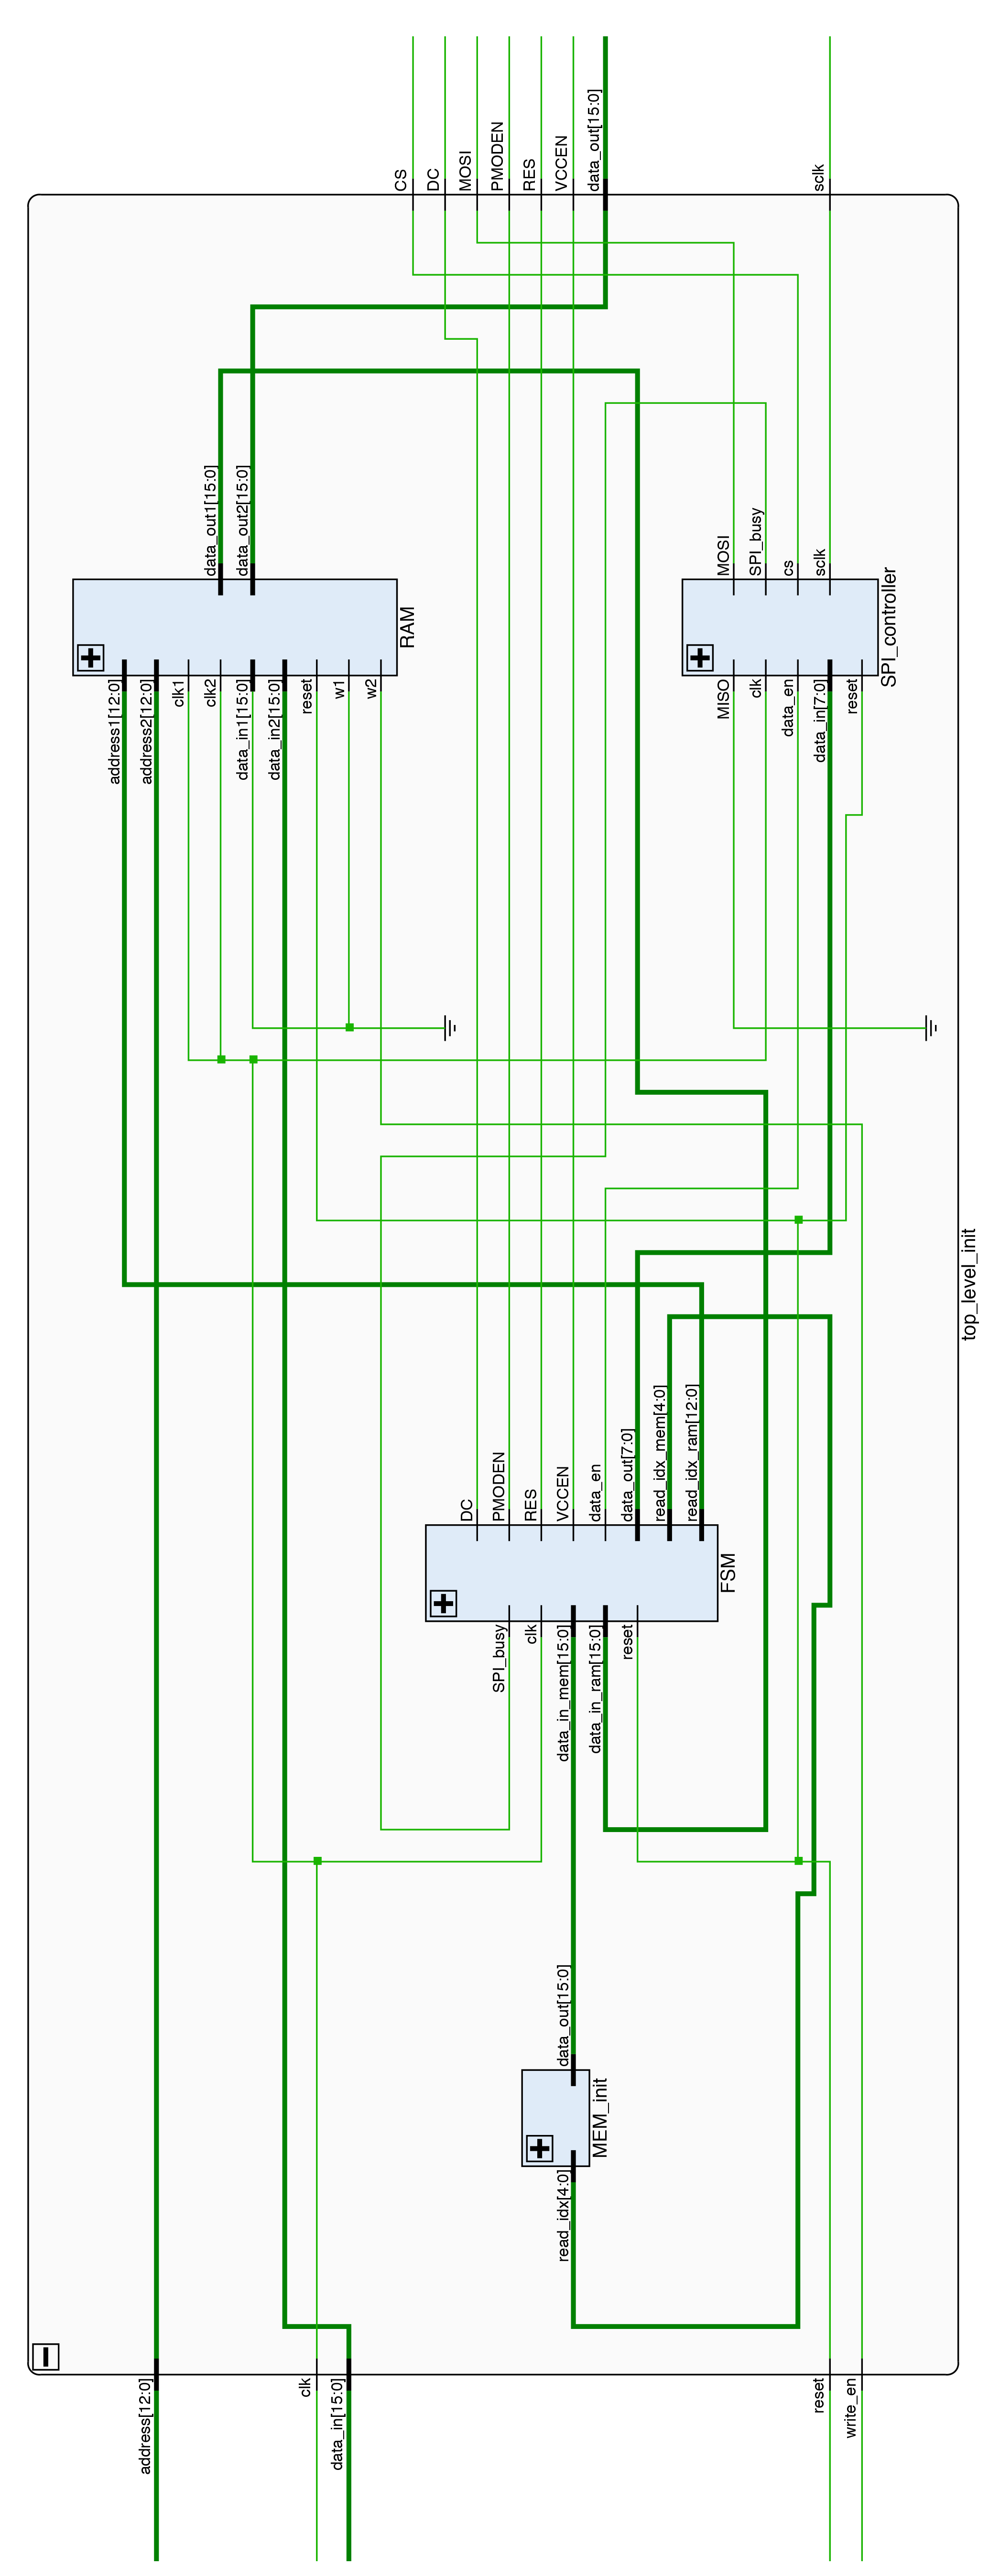
\includegraphics[scale = 1.4, keepaspectratio]{schematic_OLEDrgb_manager.png}
\caption{Schematic du module de contrôle du PMOD OLEDrgb}
\end{center}
\end{figure}

\newpage

\section{Conclusion}

%Bibliographic references
\clearpage
\begin{thebibliography}{9}
\bibitem{oleddef} 
OLED Wikipedia page for definitions\\
https://en.wikipedia.org/wiki/OLED

\bibitem{ssd1331}
Datasheet du SSD1331, contrôleur de matrice de points OLED/PLED\\
https://www.parallax.com/sites/default/files/downloads/28087-SSD1331\_1.2.pdf

\bibitem{oledrgb} 
OLEDrgb Pmod reference sheet and Datasheet\\
\textit{Pmod OLEDrgb Reference Manual.} \\
\href{https://reference.digilentinc.com/reference/pmod/pmodoledrgb/reference-manual#pinout_description_table}{https://reference.digilentinc.com/reference/pmod/pmodoledrgb/reference-manual\#pinout\_description\_table}\\
Digilent, as of January 30, 2017

\bibitem{spiimg}
Digilent SPI protocol information\\
https://reference.digilentinc.com/pmod/communication\_protocols/spi

\bibitem{spidef} 
Definition of Serial Peripherals Interface Bus and how it works\\
https://web.archive.org/web/20150413003534/http://www.ee.nmt.edu/\~teare/ee308l/datasheets/S12SPIV3.pdf\\
Motorola, Inc. , Original Release Date: January 21, 2000, Revised: February 04, 2003

\end{thebibliography}


















\end{document}